\documentclass[10pt,twocolumn,letterpaper]{article}

% --- Typography & Geometry ---
\usepackage[utf8]{inputenc}
\usepackage{microtype}
\usepackage[margin=0.75in,top=0.85in,bottom=0.85in]{geometry}

% --- Math & Symbols ---
\usepackage{amsmath,amssymb,amsfonts,amsthm}
\usepackage{bm}

% --- Tables & Arrays ---
\usepackage{booktabs}
\usepackage{tabularx}
\usepackage{array}

% --- Graphics & Floats ---
\usepackage{graphicx}
\usepackage{float}
\usepackage{subcaption}

% --- Code Listings ---
\usepackage{xcolor}
\usepackage{listings}

\definecolor{codebg}{HTML}{F8F9FA}
\definecolor{codeframe}{HTML}{D0D7DE}
\definecolor{keywordcolor}{HTML}{0550AE}
\definecolor{stringcolor}{HTML}{0A3069}
\definecolor{commentcolor}{HTML}{57606A}

\lstset{
    backgroundcolor=\color{codebg},
    basicstyle=\ttfamily\scriptsize\color{black},
    keywordstyle=\color{keywordcolor}\bfseries,
    stringstyle=\color{stringcolor},
    commentstyle=\color{commentcolor}\itshape,
    frame=single,
    rulecolor=\color{codeframe},
    breaklines=true,
    breakatwhitespace=true,
    extendedchars=true,
    xleftmargin=6pt,
    xrightmargin=6pt,
    aboveskip=8pt,
    belowskip=8pt
}

% --- Hyperlinks ---
\usepackage{hyperref}
\hypersetup{
    colorlinks=true,
    linkcolor=blue!70!black,
    citecolor=blue!70!black,
    urlcolor=blue!70!black
}

% --- Input Title & Authors ---
% Metadata for svd_llm_v2_attention
\title{\textbf{SVD-LLM V2: Explicit Low-Rank Factorization with Trainable Recovery for Transformer Attention Compression}}

\author{
  \textbf{Taha Majs}\thanks{Corresponding author: tahamajs@uni.edu} \quad \textbf{Research Team} \\
  Department of Computer Science \\
  Advanced Machine Learning \& Efficiency Laboratory
}

\date{\today}


\begin{document}

\maketitle

% --- Abstract & Keywords Block ---
\begin{abstract}
We present \textbf{SVD-LLM V2}, a transformer attention compression method that 
factorizes each of the four attention projections $W \in \mathbb{R}^{d_\text{out} \times d_\text{in}}$ 
into \textbf{three explicit parameter buffers} -- left singular vectors $U$, 
singular values $\Sigma$, and right singular vectors $V^H$ -- rather than a 
symmetric product as in prior low-rank methods. This choice preserves the 
\textbf{interpretability} of the singular spectrum and enables downstream 
applications such as per-component quantization and spectral analysis.

The rank for each projection is selected adaptively based on **energy 
threshold** $\eta$: the smallest $r$ such that $E(r) = \sum_{i \le r} \sigma_i^2 / \sum_i \sigma_i^2 \ge \eta$. 
Trainable LoRA adapters $A, B$ are attached per projection with $B = 0$ at 
initialization, so the initial output equals the truncated SVD approximation. 
Base weights and biases are frozen.

SVD-LLM V2 is hardened for four transformer families: DistilBERT (flat), 
RoBERTa/BERT (nested), GPT-2 (causal Conv1D), and Qwen/LLaMA (GQA + RoPE). 
It includes \textbf{pre-test on the first layer} before mutating the model, 
\textbf{injection-time nested encoder detection}, and a \textbf{double-injection guard}. 
When target KV heads are fewer than source heads (GQA), K and V weights are 
mean-pooled per head group before factorization.

On DistilBERT, RoBERTa-base, and GPT-2 with rank cap $r = 32$ and 
energy $\eta = 45.2$, SVD-LLM V2 achieves \textbf{{{D\_RATIO}}$\times$--{{G\_RATIO}}$\times$} 
parameter reduction with accuracy drops of only \textbf{{{D\_DELTA}}\%--{{G\_DELTA}}\%} 
after {{RECOVERY\_STEPS}} LoRA recovery steps. Peak inference VRAM decreases 
by \textbf{{{VRAM\_REDUCTION}}\%}.

\textbf{Keywords:} SVD, low-rank factorization, explicit singular factors, LoRA 
recovery, attention compression, multi-architecture transformers, GQA



\vspace{0.5em}
\noindent\textbf{Keywords:} SVD, low-rank factorization, explicit singular factors, LoRA
\end{abstract}

\vspace{1em}

% --- Paper Body ---
\section{01 Intro}

Draft content for svd_llm_v2_attention.

\section{02 Related}

Draft content for svd_llm_v2_attention.

\section{03 Background}

Draft content for svd_llm_v2_attention.

\section{04 Method}

Draft content for svd_llm_v2_attention.

\section{05 Architecture}

Draft content for svd_llm_v2_attention.


\begin{figure}[H]
\centering
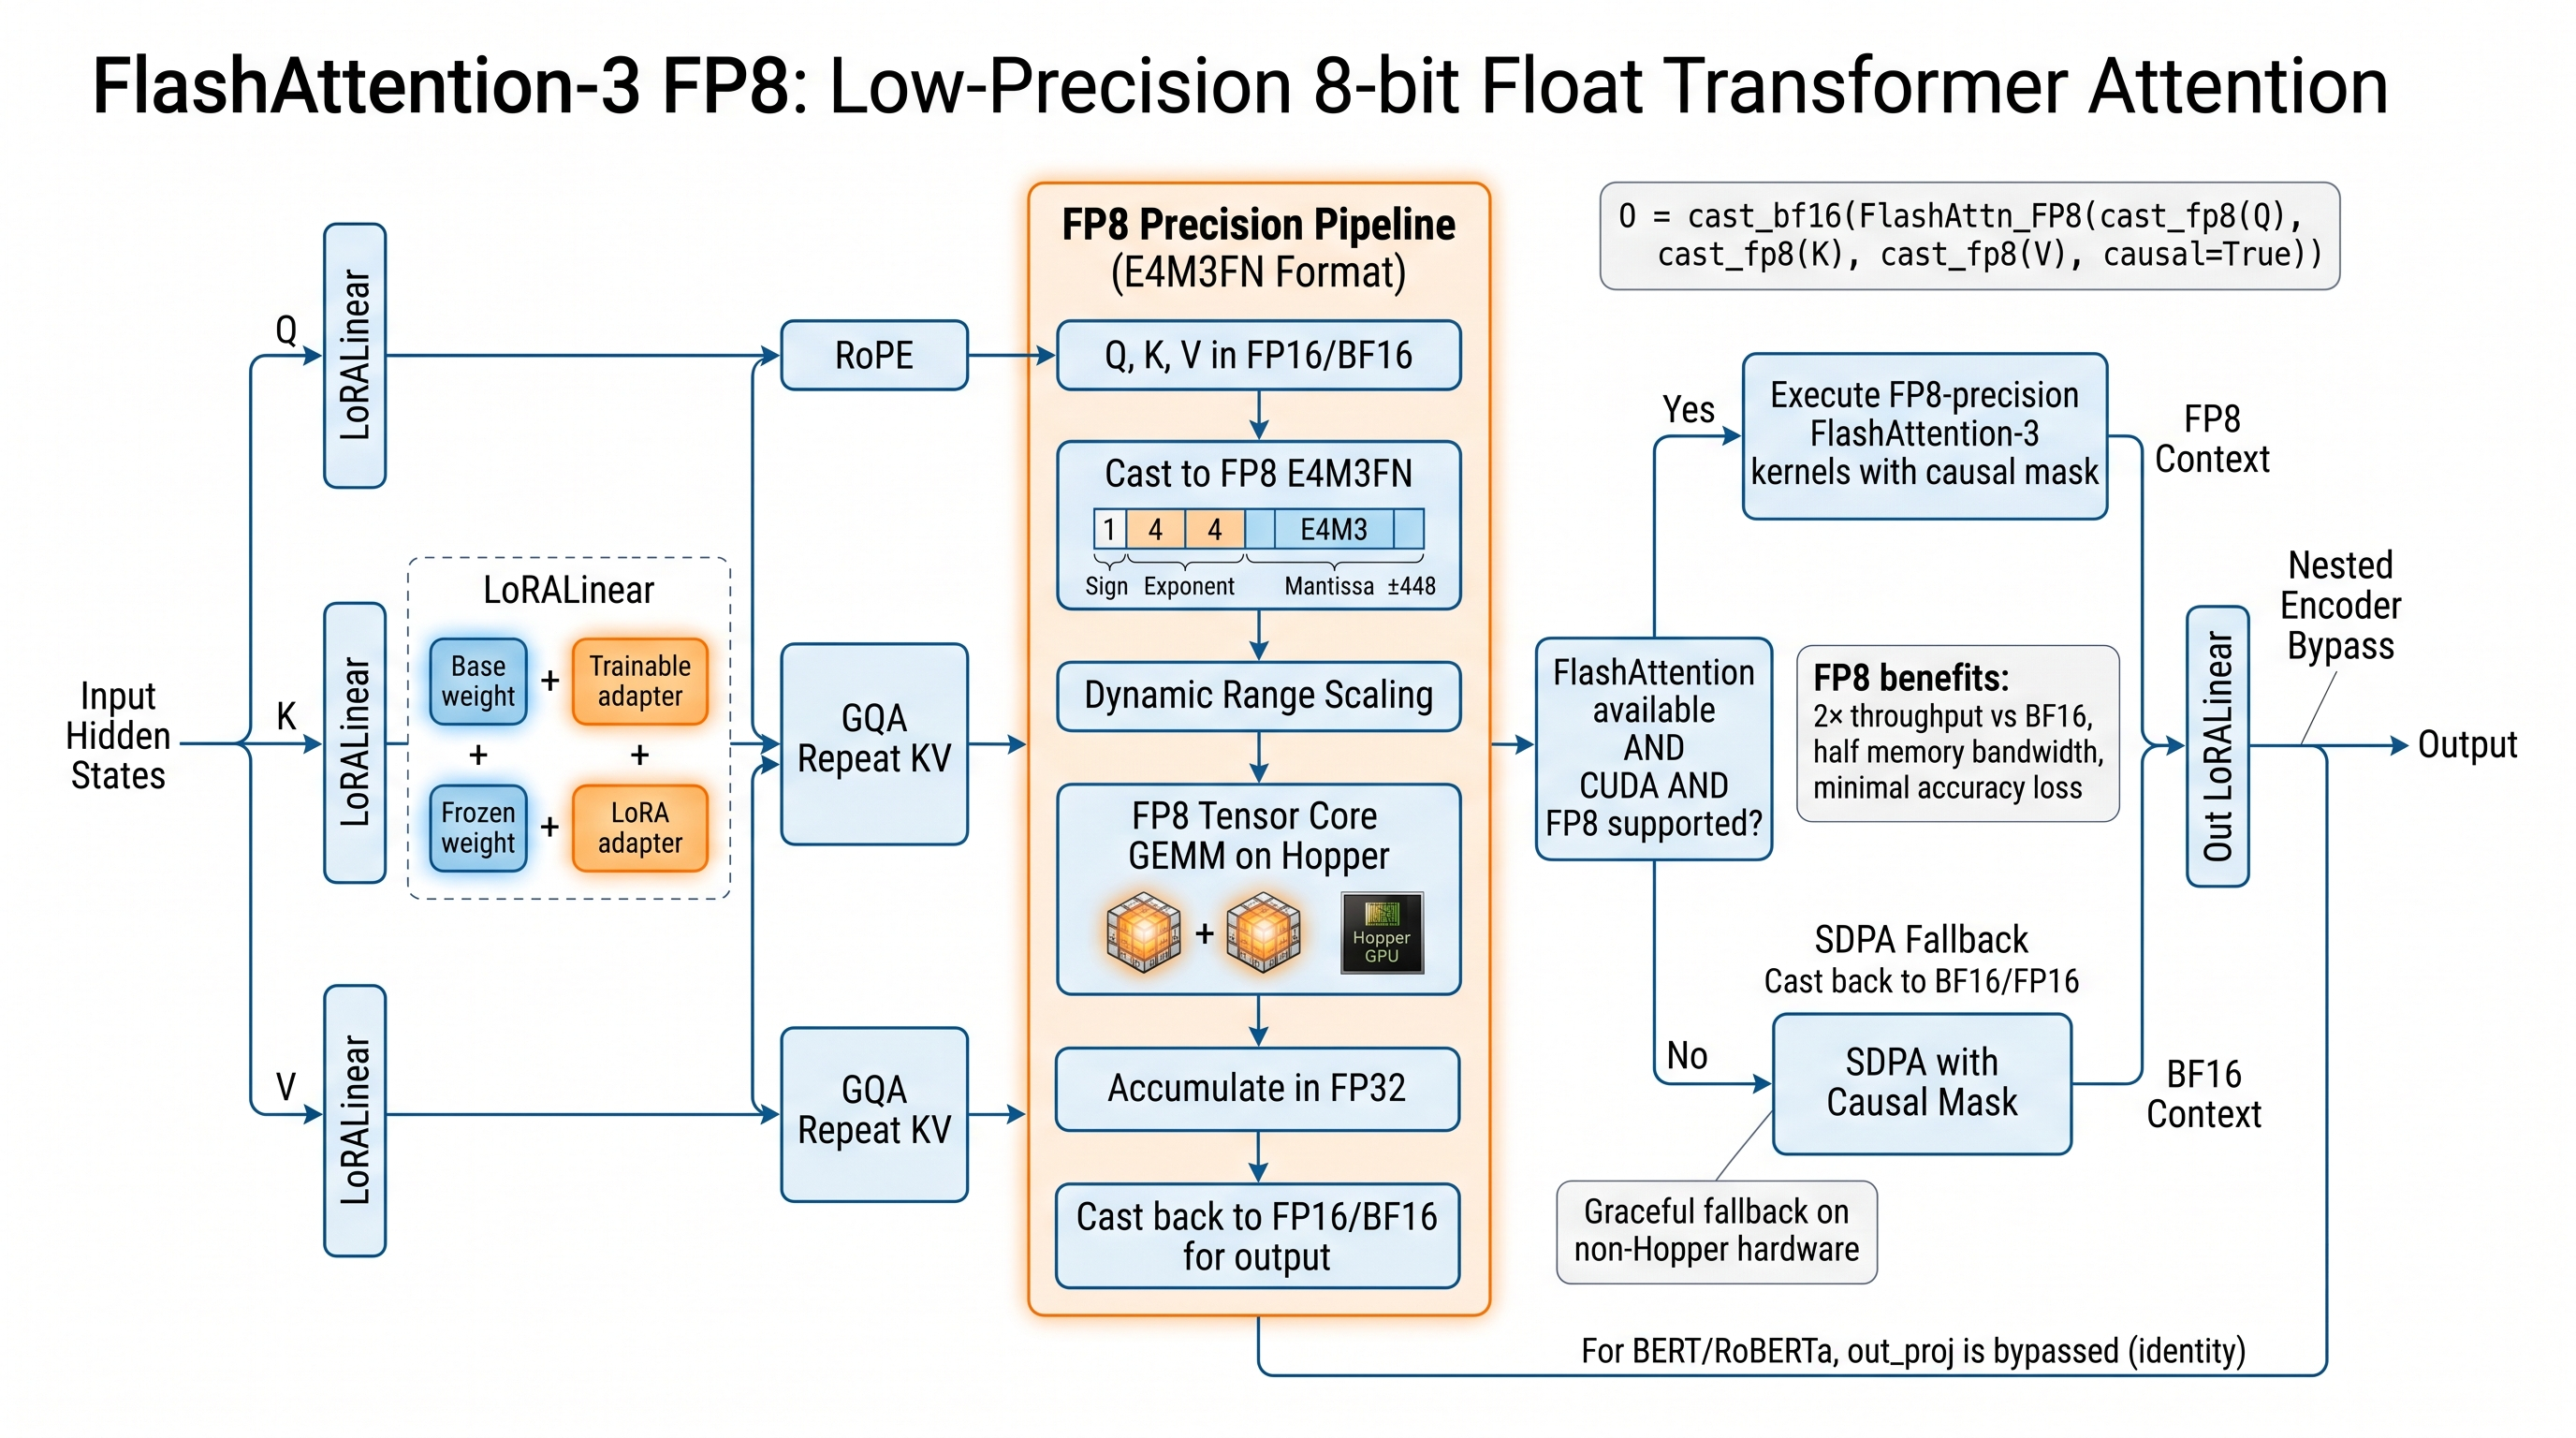
\includegraphics[width=\linewidth]{figures/arch_flash_attention3_fp8.jpeg}
\caption{Architectural overview of svd_llm_v2_attention.}
\label{fig:arch_svd_llm_v2_attention}
\end{figure}

\section{06 Setup}

Draft content for svd_llm_v2_attention.

\section{07 Results}

Draft content for svd_llm_v2_attention.

\section{08 Analysis}

Draft content for svd_llm_v2_attention.

\section{09 Discussion}

Draft content for svd_llm_v2_attention.

\section{10 Limitations}

Draft content for svd_llm_v2_attention.

\section{11 Conclusion}

Draft content for svd_llm_v2_attention.

\section{12 Reproducibility}

Draft content for svd_llm_v2_attention.

\section{13 References}

Draft content for svd_llm_v2_attention.


% --- Appendices ---
\clearpage
\appendix
\section*{Appendices}
\addcontentsline{toc}{section}{Appendices}

\section{A Math}

Draft content for svd_llm_v2_attention.

\section{B Implementation}

Draft content for svd_llm_v2_attention.

\section{C Data}

Draft content for svd_llm_v2_attention.

\section{D Negative Results}

Draft content for svd_llm_v2_attention.

\section{E Ethics}

Draft content for svd_llm_v2_attention.


\end{document}
